\chapter{Component wear anomalies: Skin wrapper machines}


\section{Data}

The dataset represents a single run-to-failure experiment of a skin wrapper machine with a 4 ms sampling period and different segments (i.e., operating mode).

\begin{figure}[H]
    \centering
    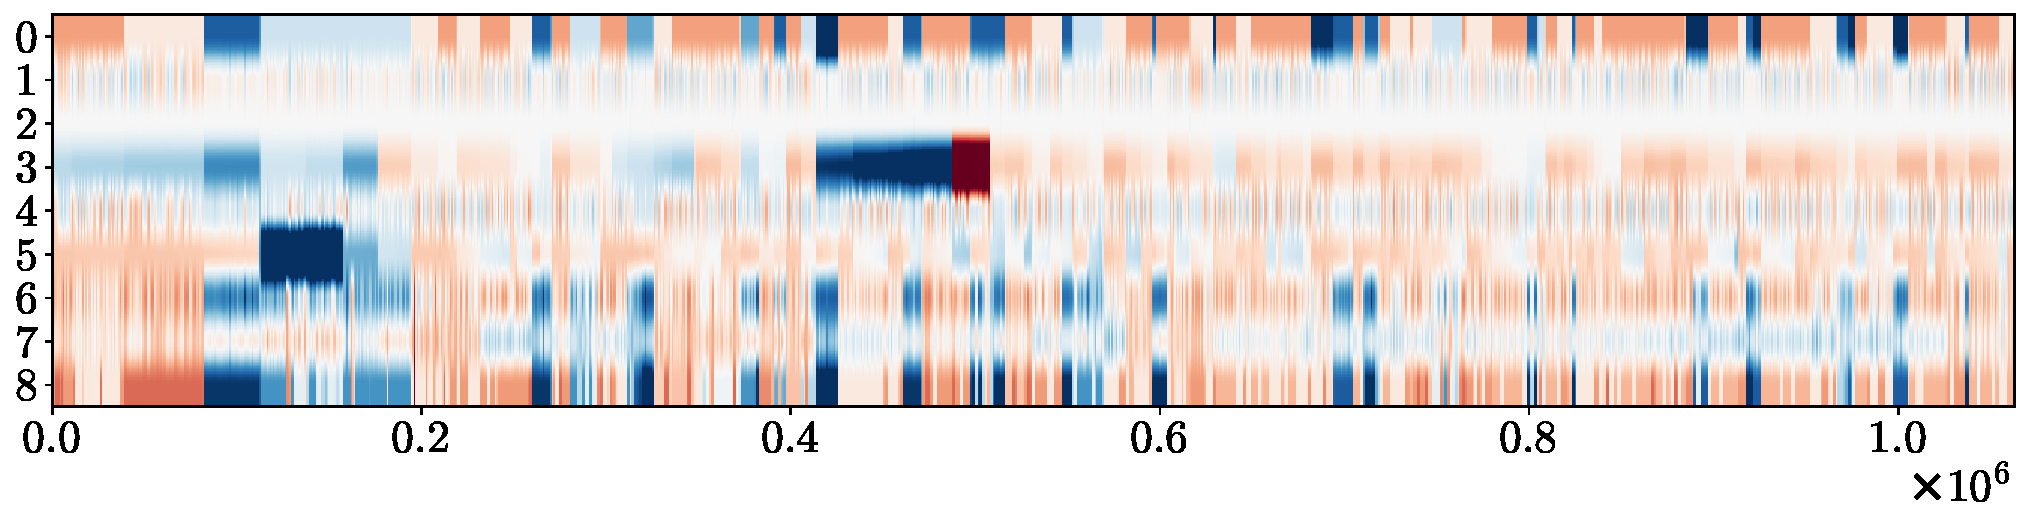
\includegraphics[width=0.9\linewidth]{./img/_skinwrapper_heatmap.pdf}
    \caption{Dataset heatmap}
\end{figure}

The following observations can be made:
\begin{itemize}
    \item Some features (i.e., rows 0 and 8 of the heatmap) are fixed for long periods of time (i.e., piece-wise constant). They are most likely controlled parameters.
    \begin{figure}[H]
        \centering
        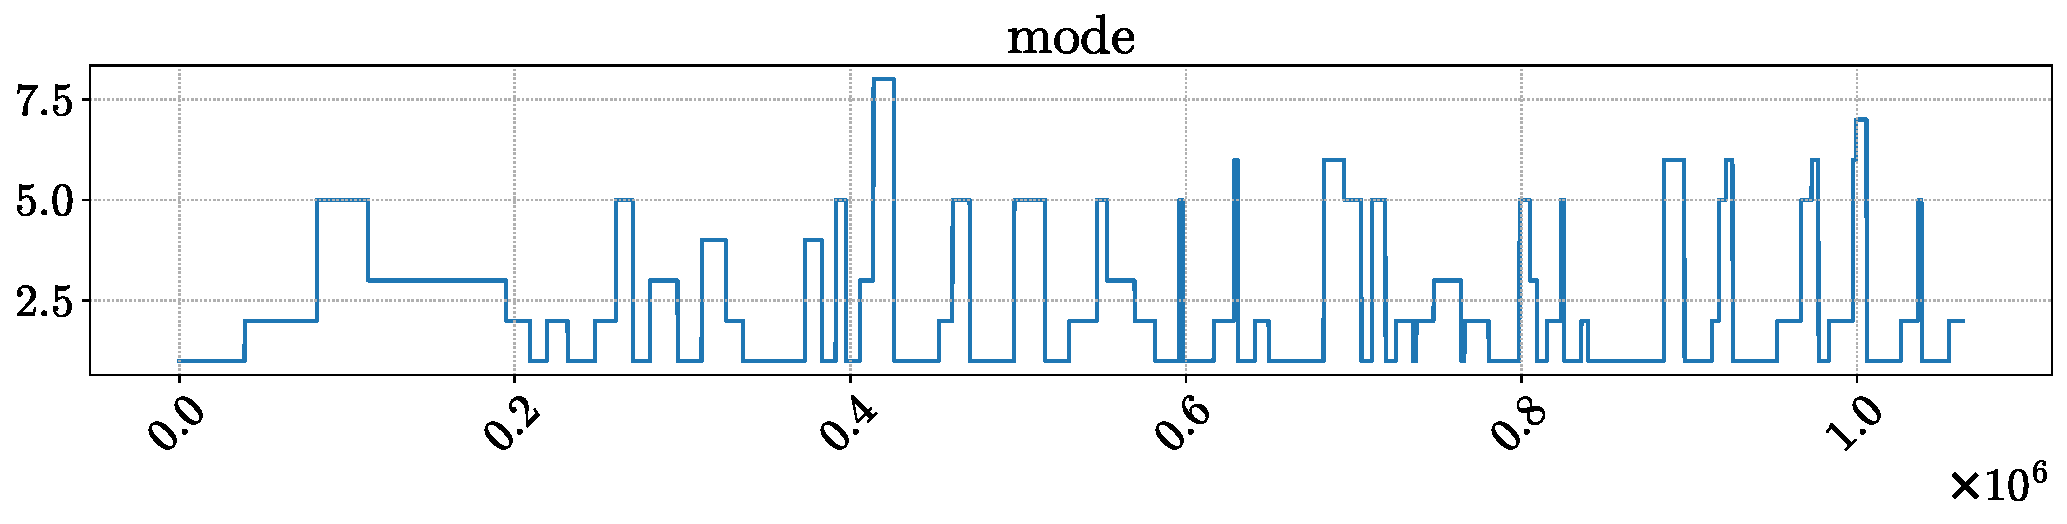
\includegraphics[width=0.8\linewidth]{./img/_skinwrapper_constant.pdf}
    \end{figure}

    \item A feature (i.e., row 2 of the heatmap) seems constant but in reality it has many short-lived peaks.
    \begin{figure}[H]
        \centering
        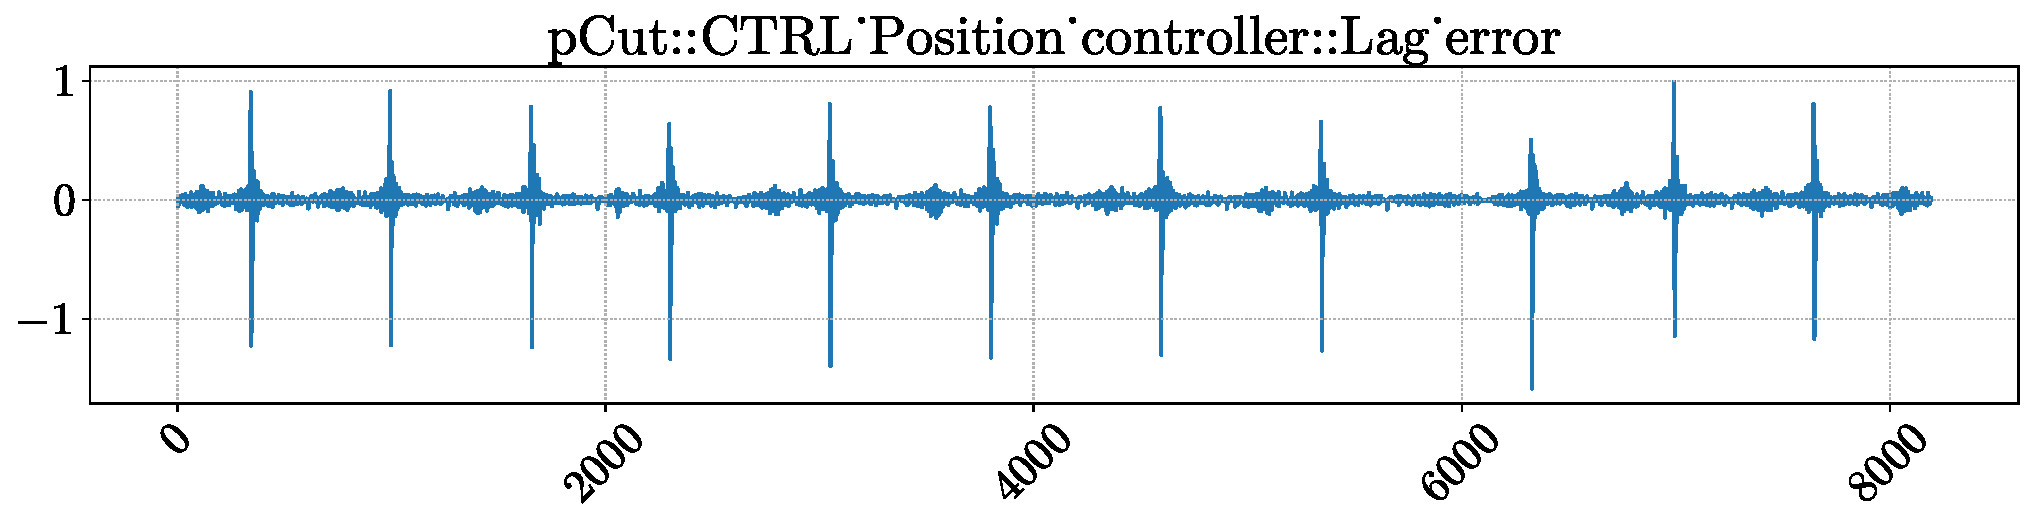
\includegraphics[width=0.8\linewidth]{./img/_skinwrapper_peaks.pdf}
    \end{figure}

    \begin{remark}
        This type of signal might be useful to determine a period in the series.
    \end{remark}

    \item Some features (i.e., rows 3 and 5 of the heatmap) contain sudden localized deviations. This is most likely due to external interventions.
    \begin{figure}[H]
        \centering
        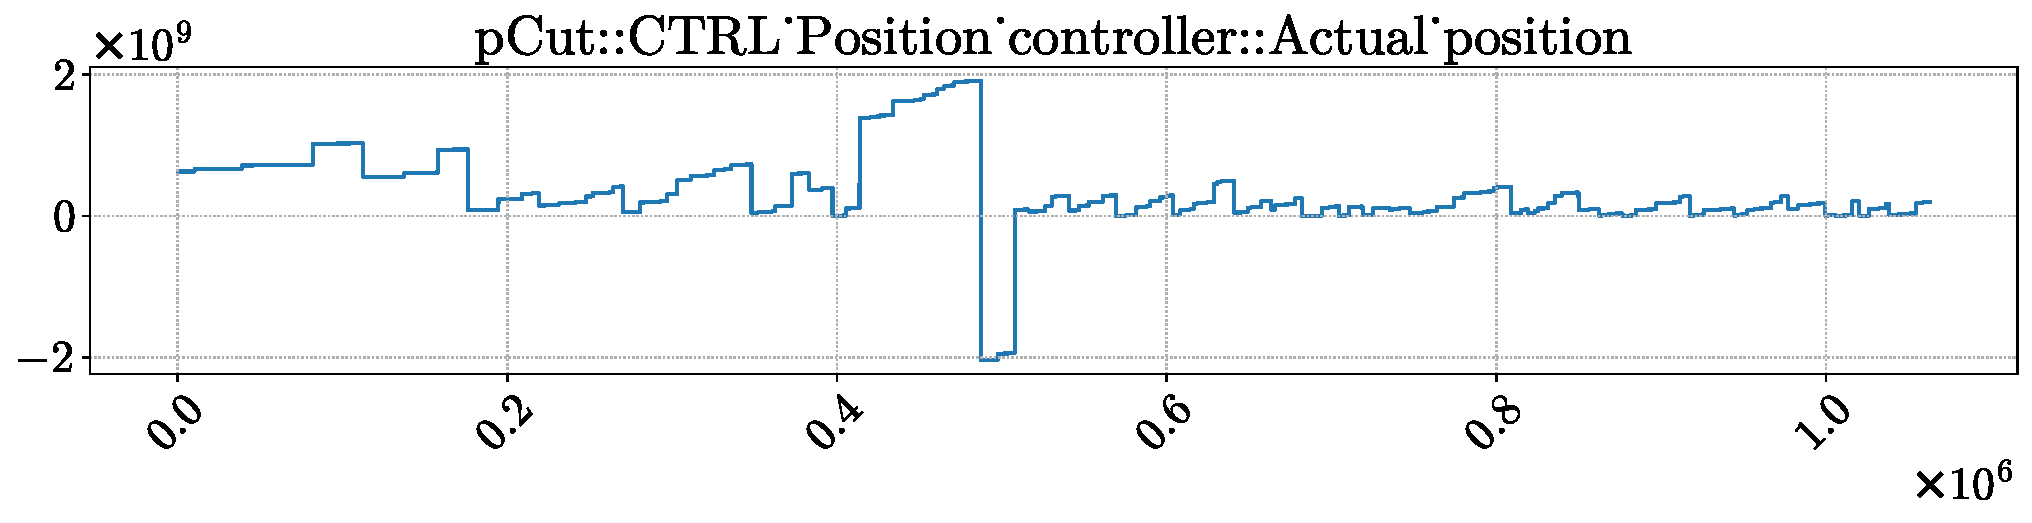
\includegraphics[width=0.8\linewidth]{./img/_skinwrapper_deviation.pdf}
    \end{figure}
\end{itemize}


\subsection{Binning}

\begin{description}
    \item[Binning] \marginnote{Binning}
        Reduce the granularity of the data using a non-overlapping sliding window and aggregation functions.

        \begin{remark}
            With high-frequency data, some approaches (e.g., a neural network) might not be able to keep up if real-time predictions are required.
        \end{remark}

        \begin{remark}
            After binning, the number of samples is reduced, but the number of features might increase.
        \end{remark}
\end{description}



\section{Approaches}


\subsection{Autoencoder}

\begin{description}
    \item[Autoencoder]
        Train an autoencoder on earlier non-anomalous data and use the reconstruction error to detect component wear.

        Results show that there is a high reconstruction error for the operating mode feature (i.e., first row), which is a controlled parameter. This hints at the fact that some operating modes are too infrequent, so the model is unable to reconstruct them.
        \begin{figure}[H]
            \centering
            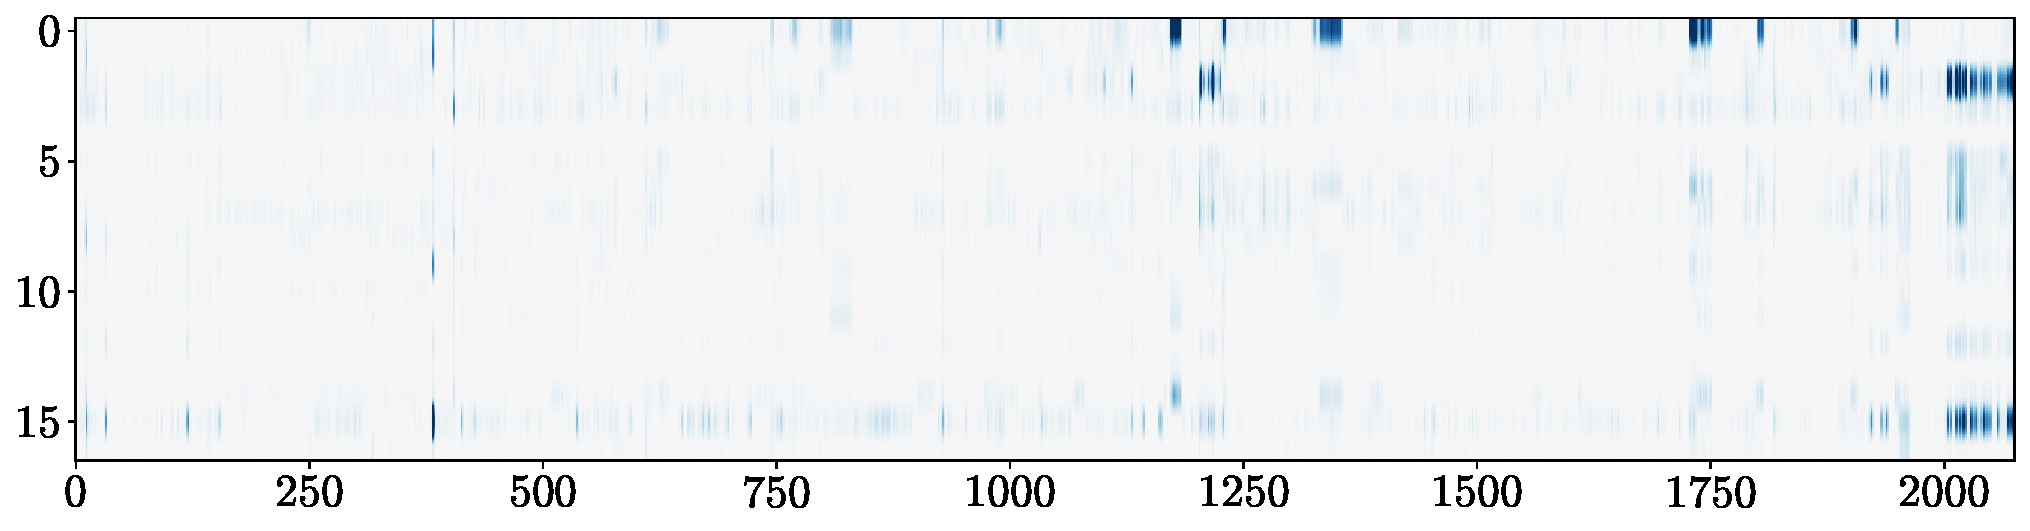
\includegraphics[width=0.9\linewidth]{./img/_skinwrapper_autoencoder.pdf}
        \end{figure}

\end{description}

\begin{remark}
    There is a distribution drift (i.e., future does not behave like the past) in the dataset.

    \begin{figure}[H]
        \centering
        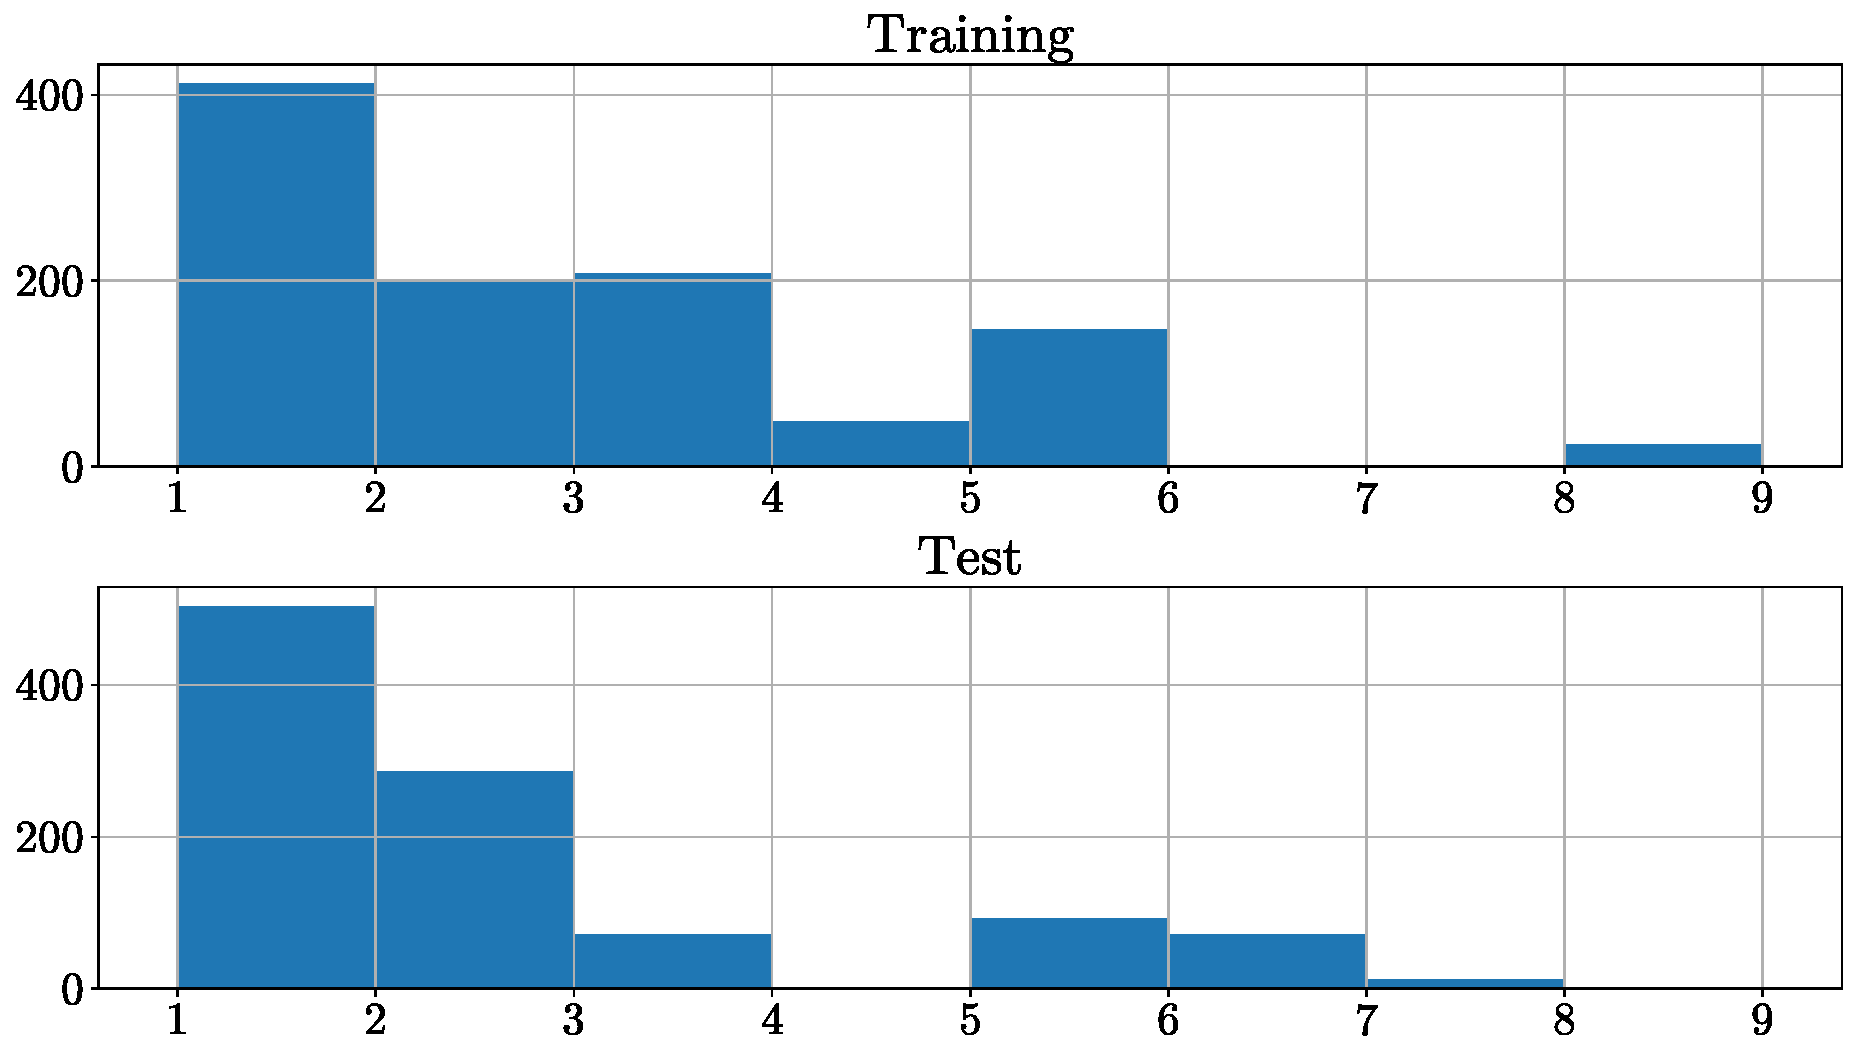
\includegraphics[width=0.65\linewidth]{./img/_skinwrapper_distribution.pdf}
    \end{figure}
\end{remark}

\begin{remark}
    To account for distribution drift, chronological splitting for the training and test sets is a better approach instead of random sampling (which ignores the drift).

    The validation set can be created through random sampling as, in case it is created chronologically, it might create a gap between training and test data. However, this approach ignores drift when validating.
\end{remark}


\subsection{Class rebalancing}


\begin{remark}
    Consider two training samples $\{ (x_1, y_1), (x_2, y_2) \}$, the optimization problem over an objective function $f_\theta$ would be:
    \[
        \arg\max_\theta f_\theta(y_1 | x_1) f_\theta(y_2 | x_2)
    \]
    If the second sample $(x_2, y_2)$ appears twice, the problem is:
    \[
        \begin{split}
            &\arg\max_\theta f_\theta(y_1 | x_1) f_\theta(y_2 | x_2)^2 \\
            &= \arg\max_\theta f_\theta(y_1 | x_1)^{\frac{1}{3}} f_\theta(y_2 | x_2)^{\frac{2}{3}}
        \end{split}
    \]
\end{remark}

\begin{description}
    \item[Importance sampling] \marginnote{Importance sampling}
        Given an empirical risk minimization problem:
        \[ \arg\min_\theta - \prod_{i=1}^{m} f_\theta(y_i | x_i) \]
        Each training sample can have associated a different weight $w_i$:
        \[ 
            \begin{split}
                &\arg\min_\theta - \prod_{i=1}^{m} f_\theta(y_i | x_i)^{w_i} \\
                &= \arg\min_\theta - \sum_{i=1}^{m} w_i \log\left( f_\theta(y_i | x_i) \right)
            \end{split}
        \]

        The weights can be seen as a ratio:
        \[ w_i = \frac{p_i^*}{p_i} \]
        where:
        \begin{itemize}
            \item $p_i$ is the sampling bias that has to be canceled out.
            \item $p_i^*$ is the target distribution to emulate.
        \end{itemize}
\end{description}

In this problem, we can define the weights as follows:
\[
    \begin{split}
        p_i &= \frac{1}{n} | \text{samples with the same operating mode as $x_i$} | \\
        p_i^* &= \frac{1}{n}
    \end{split}
\]

\begin{remark}
    As uniform distribution is assumed, the detector will not be sensitive to the mode.
\end{remark}

\begin{figure}[H]
    \centering
    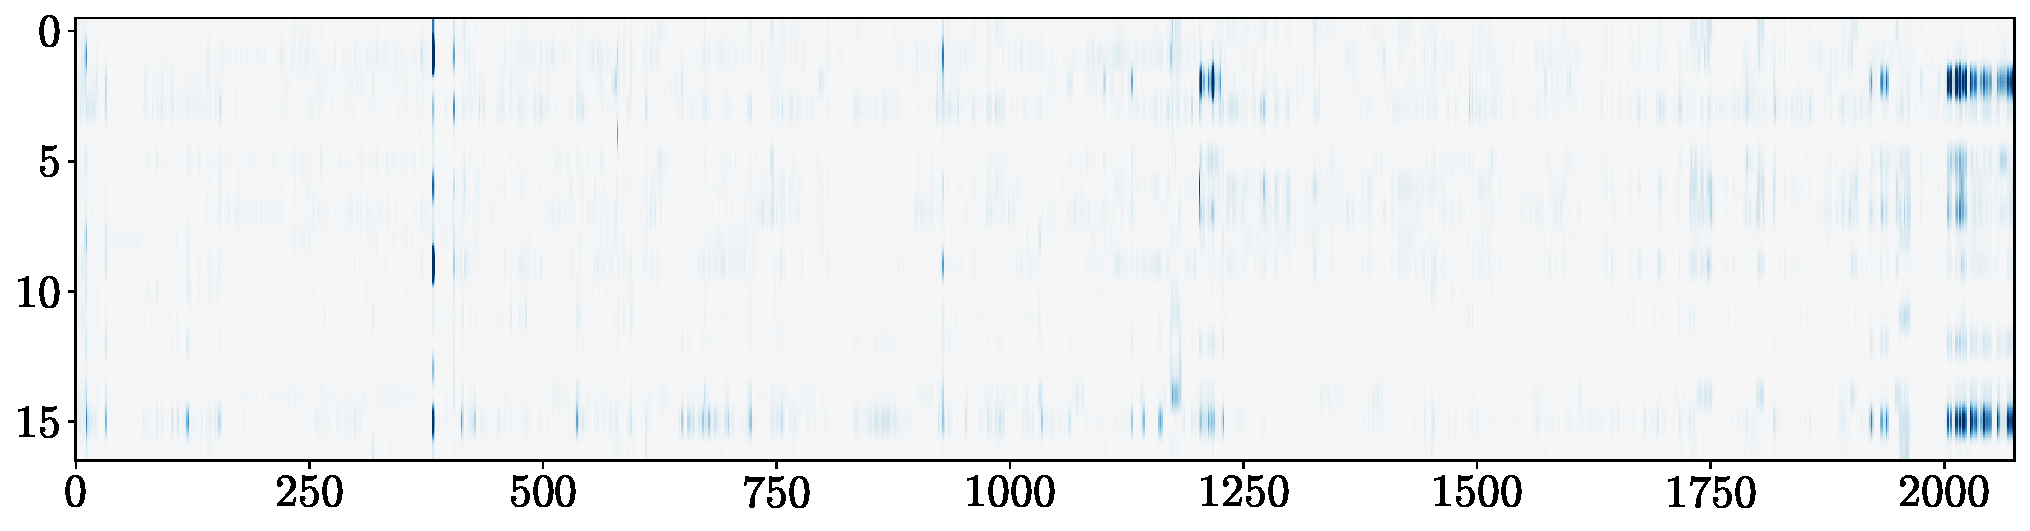
\includegraphics[width=0.9\linewidth]{./img/_skinwrapper_importance.pdf}
    \caption{
        \parbox[t]{0.7\linewidth}{
            Autoencoder feature reconstruction error with importance sampling. Note that the operation mode (row 0) now has fewer errors.
        }
    }
\end{figure}

\subsubsection{Importance sampling applications}

\begin{description}
    \item[Class rebalancing]
        Oversample or undersample training samples based on the class unbalance.

        \begin{remark}
            When evaluating a model trained on a rebalanced training set, accuracy might not be the ideal metric. A cost model or confusion matrix can be used.
        \end{remark}

        \begin{remark}
            Rebalancing should not be used when the data is unbalanced but representative of the real distribution.
        \end{remark}

    \item[Remove bias from continuous attributes]
        $p_i$ and $p_i^*$ can be probability densities. Therefore, with a continuous feature, it is sufficient to estimate $p_i$ using a density estimator.

        \begin{remark}
            It can be useful to clip $p_i$ for numerical stability:
            \[ p_i = \max(l, \min(u, f(x_i, y_i))) \]
        \end{remark}

    \item[Remove bias from external attributes]
        If the dataset is generated from biased external sources, it is possible to attempt to debias it by determining the probability that a sample belong to the dataset and use it as $p_i$.

        \begin{example}
            A dataset for organ transplants already contains patients for which doctors think the surgery is more likely to be successful.

            $p_i$ can be the probability that the patient has been selected to be an organ receiver.
        \end{example}

    \item[Sample-specific variance]
        Importance sampling applied with MSE allows to remove its homoscedasticity (i.e., allow non-constant variance).

        Consider MSE formulated as follows:
        \[ \arg\min_\theta - \sum_{i=i}^{m} \log\left( \frac{1}{\sqrt{2\pi}} \exp\left( -\frac{1}{2}(y_i - h_\theta(x_i))^2 \right) \right) \]
        By adding as weights $\frac{1}{\hat{\sigma}_i^2}$, the problem becomes:
        \[ 
            \begin{split}
                &\arg\min_\theta - \sum_{i=i}^{m} \frac{1}{\hat{\sigma}_i^2} \log\left( \frac{1}{\sqrt{2\pi}} \exp\left( -\frac{1}{2}(y_i - h_\theta(x_i))^2 \right) \right) \\
                &= \arg\min_\theta - \sum_{i=i}^{m} \log\left( \frac{1}{\sqrt{2\pi}} \exp\left( -\frac{(y_i - h_\theta(x_i))^2}{2\hat{\sigma}_i^2} \right) \right) \\
            \end{split}
        \]
        In other words, the weight in the form $\frac{1}{\hat{\sigma}_i^2}$ represents the inverse sample variance. Therefore, it is possible to specify a different variance for each sample.
\end{description}